%
% k-geodaeten.tex -- Gleichung der Geodäten, Christoffel-Symbole
%
% (c) 2017 Prof Dr Andreas Müller, Hochschule Rapperswil
%
\chapter{Geodäten
\label{skript:chapter:geodaeten}}
\lhead{Geodäten}
\rhead{}
In der Ebene ist die kürzeste Verbindung zwischen zwei Punkten
eine Gerade.
Auf einem Zylinder oder Kegel kann man die kürzeste Verbindung finden,
indem man die Fläche in eine Ebene abrollt, und dann dort verwendet,
dass die kürzeste Verbindung in der Ebene eine Gerade ist.
Dies zeigt, dass die kürzesten Verbindung nichts mit der speziellen
Einbettung einer Fläche zu tun hat, sondern eine Eigenschaft ist,
die sich allein aus der Längenmessung in der Fläche ist, man nennt
dies auch eine intrinsische Eigenschaft.

Auf einer Kugeloberfläche kann man die kürzesten Verbindungen ebenfalls
direkt angeben, es sind die Grosskreise.
\begin{figure}
\centering
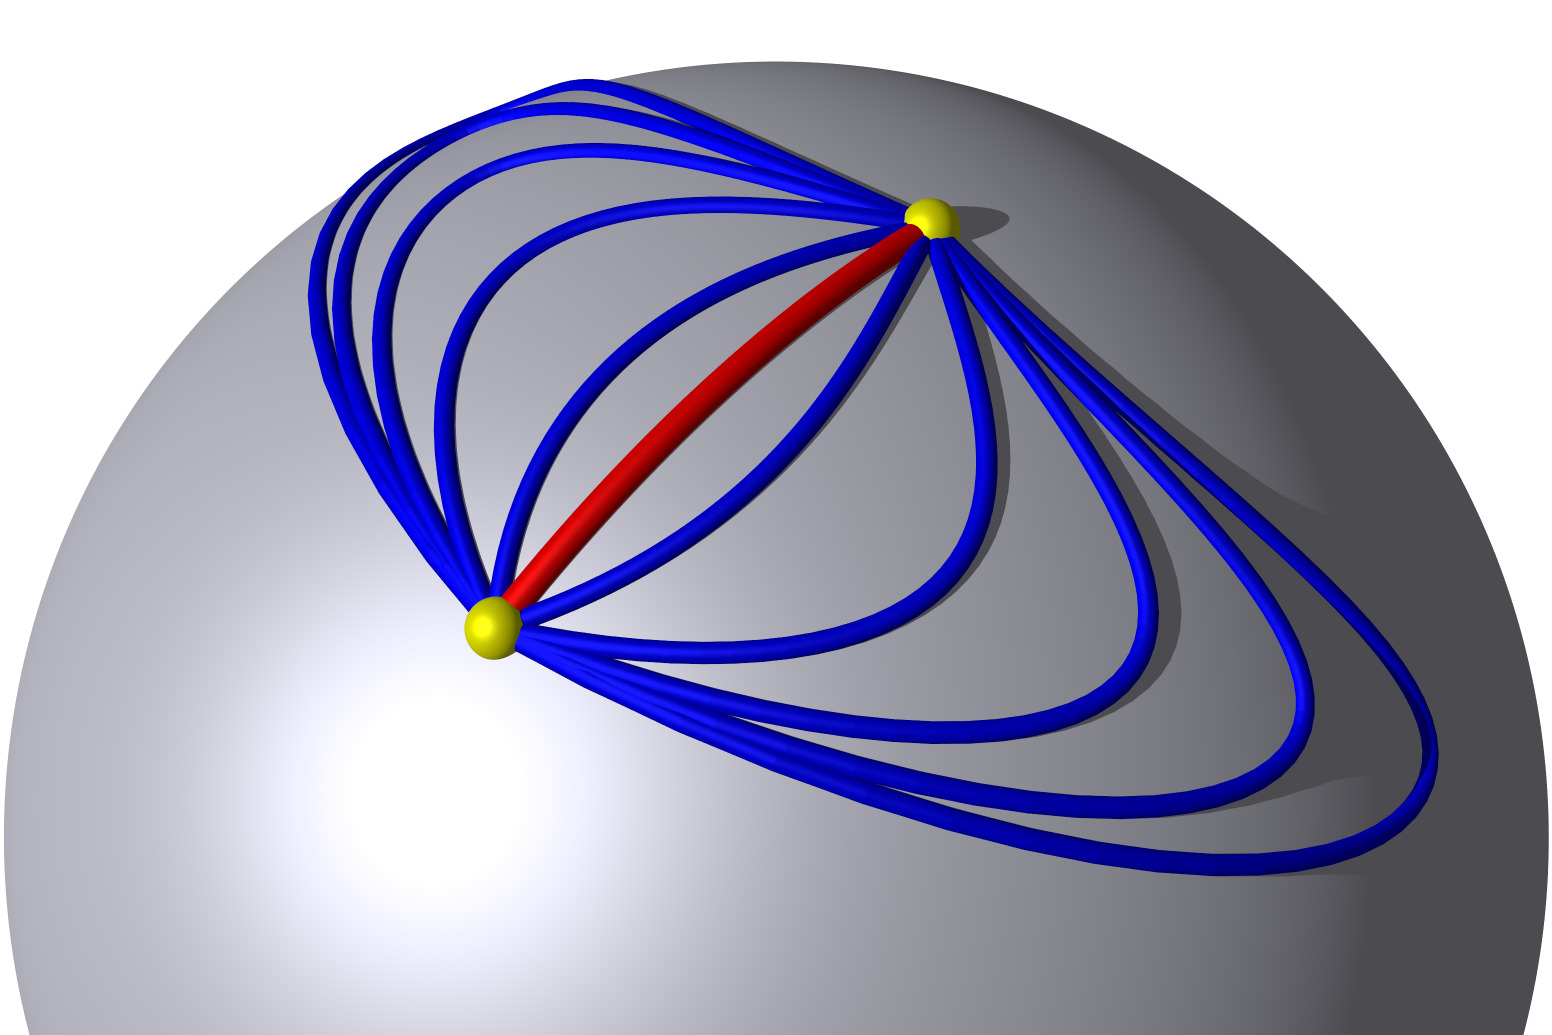
\includegraphics[width=\hsize]{chapters/3d/geodaete.jpg}
\caption{Ein Ausschnitt aus einem Grosskreis (rot) ist die kürzestmögliche
Verbindung zwischen zwei Punkten auf einer Kugeloberfläche.
Alle anderen Kurven (blau) in der Kugeloberfläche haben grössere Länge.
\label{skript:kruemmung:fig:geodaete}}
\end{figure}
Man kann dabei so argumentieren: von allen Schnitten der Kugeloberfläche
mit Ebenen durch die zwei gegeben Punkte ist der Grosskreis derjenige
mit der kleinsten Krümmung, und daher die ``direkteste'' Verbindung.
Dieses Argument ist allerdings nicht ganz exakt, denn man vergisst dabei,
dass es noch viele weitere Kurven gibt, die die beiden Punkte verbinden
(Abbildung~\ref{skript:kruemmung:fig:geodaete}).
Es ist auch nicht wirklich auf noch allgemeinere Situationen übertragbar,
denn es nützt aus, dass die Kugeloberfläche homogen ist, in jedem Punkt
ist die ``Krümmung'' (ein im Moment noch nicht definierter Begriff) 
gleich gross.

Auch die Ausbreitung des Lichts in einem Medium ist einer solchen
Beschreibung zugänglich.
Das Licht wählt immer den Weg mit der geringsten Laufzeit, nicht
unbedingt den geometrisch kürzesten Weg.
Daher können sich Lichtstrahlen in einem inhomogenen Medium
krümmen.
Aus der Perspektive des Lichtes ist aber nicht die Bahn gekrümmt,
es folgt der in dieser Geometrie geradest möglichen Bahn.
Nicht die Bahn ist gekrümmt, sondern die Längenmessung weicht von
der üblichen \eqref{skript:kruemmung:pytagoras} ab, der Raum ist
gekrümmt.

In diesem Abschnitt suchen wir daher nach einer allgemeinen Methode,
die kürzeste Verbindung, die sogenannten Geodäten zu finden.

\section{Paralleltransport}
\rhead{Paralleltransport}
Die Beispiele von kürzesten Verbindungen suggerieren, dass die kürzeste
Verbindung auch die ``geradeste'' ist, sie weicht möglichst wenig von
der Richtung des aktuellen Tangentialvektors ab.
Das Problem bei dieser Interpretation ist allerdings, dass wir Vektoren
in zwei verschiedenen Punkten der Fläche nicht unmittelbar vergleichen
können.
Auf der Kugeloberfläche liegen die Tangentialvektoren an eine Kurve in
verschiedenen Punkten zum Beispiel in verschiedenen Tangentialebenen
an die Kugel.

Wir müssen also zunächst in der Lage sein, Vektoren in zwei verschiedenen
Punkten miteinander zu vergleichen.
Wir können das tun, indem wir einen Vektor entlang einer Kurve transportieren,
wobei wir versuchen, in so parallel zu sich selbst wie möglich zu sich
selbst zu halten.
Auch dies ist im Moment noch ein etwas schwammiger Begriff. 
Es ist aber klar, dass die Komponenten des transportierten Vektors
sowohl von der Transportrichtung wie auch vom ursprünglichen Vektor
abhängen.
Seien $A^\mu$ die Komponenten eines Vektors, die Richtung mit Komponenten
$\Delta x^\nu$ transport werden soll.
Dann wird der transportierte die Form
\[
\tilde A^\alpha
=
A^\alpha - \Gamma_{\mu\nu}^\alpha A^\mu \Delta x^\nu
\]
haben.
Die Wahl des Vorzeichens von $\Gamma_{\mu\nu}^\alpha$ ist im Wesentlichen
eine Frage der Konvention.
Die instantane Änderung zur Zeit $t=0$ entlang der Kurve ist
\begin{equation}
\frac{d}{dt}\tilde A^\alpha\bigg|_{t=0}
=
\Gamma_{\mu\nu}^\alpha A^\mu \dot x^\nu.
\label{skript:kruemmung:ableitung}
\end{equation}

Bis jetzt haben wir die Metrik nicht verwendet.
Wir möchten dass der Paralleltransport die Länge des Vektors beim
Transport entlang einer Kurve nicht verändert.
Die Länge des Vektors wird durch $g_{\mu\nu}\tilde A^\mu \tilde A^\nu$
gegeben.
Die Ableitung entlang der Kurve $x^\mu(t)$ ist
\[
\frac{d}{dt} g_{\mu\nu}\tilde A^\mu \tilde A^\nu\bigg|_{t=0}
=
\frac{\partial g_{\mu\nu}}{\partial x^\alpha}A^\mu A^\nu\dot x^\alpha
-
g_{\mu\nu}A^\mu\Gamma_{\alpha\beta}^\nu A^\alpha \dot x^\beta
-
g_{\mu\nu}\Gamma_{\alpha\beta}^\mu A^\alpha \dot x^\beta A^\nu
=
0.
\]
In diesem Ausdruck kommen in allen Termen $A^\mu$ und $\dot x^\beta$ mit
verschiedenen Indizes vor.
Damit wir diese Faktoren ausklammern können, nennen wir die Indizes um,
so dass sie in allen Termen gleich sind.
Wir erhalten dann die Gleichung
\[
\biggl(
\frac{\partial g_{\mu\nu}}{\partial x^\alpha}
-
g_{\mu\beta}\Gamma_{\nu\alpha}^\beta
-
g_{\beta\nu}\Gamma_{\mu\alpha}^\beta
\biggr)
A^\mu A^\nu\dot x^\alpha
=
0
\]
F"ur die Koeffizienten $\Gamma$.
Diese Gleichung muss f"ur jede beliebige Wahl von $A^\mu$ und jede
beliebige Richtung der Kurve $\dot x^\alpha$ erfüllt sein, wenn der
Klammerausdruck verschwindet für alle Werte der freien, also nicht durch
die Summationskonvention als Laufindizes ausgezeichneten, Indizes.
Wir erhalten also
\[
\frac{\partial g_{\mu\nu}}{\partial x^\alpha}
-
g_{\mu\beta}\Gamma_{\nu\alpha}^\beta
-
g_{\beta\nu}\Gamma_{\mu\alpha}^\beta
=
0,
\]
ein System von Gleichungen für die $n^3$ Grössen $\Gamma_{\mu\nu}^\alpha$.
Wir können die $\Gamma$ auch allein auf der linken Seite haben:
\[
g_{\mu\beta}\Gamma_{\nu\alpha}^\beta
+
g_{\beta\nu}\Gamma_{\mu\alpha}^\beta
=
\frac{\partial g_{\mu\nu}}{\partial x^\alpha}
\]
Durch zyklische Vertauschung der drei Indizes $\mu$, $\nu$ und $\alpha$
erhalten wir drei Gleichungen
\[
\def\arraystretch{2.0}
\begin{linsys}{3}
g_{\mu\beta}\Gamma_{\nu\alpha}^\beta &+& g_{\beta\nu}\Gamma_{\mu\alpha}^\beta
& &
&=&
\displaystyle
\frac{\partial g_{\mu\nu}}{\partial x^\alpha}
\\
& &g_{\nu\beta}\Gamma_{\alpha\mu}^\beta &+& g_{\beta\alpha}\Gamma_{\nu\mu}^\beta
&=&
\displaystyle
\frac{\partial g_{\nu\alpha}}{\partial x^\mu}
\\
g_{\beta\mu}\Gamma_{\alpha\nu}^\beta
& &
&+&g_{\alpha\beta}\Gamma_{\mu\nu}^\beta 
&=&
\displaystyle
\frac{\partial g_{\alpha\mu}}{\partial x^\nu}
\end{linsys}
\]
Da sowohl $g$ als auch $\Gamma$ in den unteren Indizes symmetrisch
sind, können wir die Gleichungen weiter vereinfachen:
\[
\def\arraystretch{2.0}
\begin{linsys}{3}
g_{\mu\beta}\Gamma_{\nu\alpha}^\beta
	&+& g_{\nu\beta}\Gamma_{\mu\alpha}^\beta
		& &
&=&
\displaystyle
\frac{\partial g_{\mu\nu}}{\partial x^\alpha}
\\
	& &g_{\nu\beta}\Gamma_{\mu\alpha}^\beta
		&+& g_{\alpha\beta}\Gamma_{\nu\mu}^\beta
&=&
\displaystyle
\frac{\partial g_{\nu\alpha}}{\partial x^\mu}
\\
g_{\mu\beta}\Gamma_{\nu\alpha}^\beta
	& &
		&+&g_{\alpha\beta}\Gamma_{\nu\mu}^\beta 
&=&
\displaystyle
\frac{\partial g_{\alpha\mu}}{\partial x^\nu}
\end{linsys}
\]
Subtrahieren wir die erste Zeile von der Summe der letzten beiden,
heben sich ersten Terme weg, es bleibt
\[
g_{\alpha\beta}\Gamma_{\nu\mu}^\beta
=
\biggl(
\frac{\partial g_{\nu\alpha}}{\partial x^\mu}
+
\frac{\partial g_{\alpha\mu}}{\partial x^\nu}
-
\frac{\partial g_{\mu\nu}}{\partial x^\alpha}
\biggr).
\]
Bezeichen wir die inverse Matrix von $g_{\alpha\beta}$ mit
$g^{\alpha\beta}$, dann k"onnen wir nach $\Gamma_{\mu\nu}^\beta$ aufl"osen:
\[
g^{\sigma\alpha}
\biggl(
\frac{\partial g_{\nu\alpha}}{\partial x^\mu}
+
\frac{\partial g_{\alpha\mu}}{\partial x^\nu}
-
\frac{\partial g_{\mu\nu}}{\partial x^\alpha}
\biggr)
=
g^{\sigma\alpha}
g_{\alpha\beta}\Gamma_{\mu\nu}^\beta
=
\delta^\sigma_\beta\Gamma_{\mu\nu}^\beta
=
\Gamma_{\mu\nu}^\sigma.
\]

\begin{definition}
Sei $g_{\mu\nu}$ ein metrischer Tensor. 
Dann heissen die
\[
\Gamma_{\alpha,\mu\nu}
=
\frac12
\biggl(
\frac{\partial g_{\nu\alpha}}{\partial x^\mu}
+
\frac{\partial g_{\alpha\mu}}{\partial x^\nu}
-
\frac{\partial g_{\mu\nu}}{\partial x^\alpha}
\biggr)
\]
die {\em Christoffelsymbole 1.~Art}
und
\[
\Gamma_{\mu\nu}^\sigma
=
g^{\sigma\alpha} \Gamma_{\alpha,\mu\nu}
=
\frac12
g^{\sigma\alpha}
\biggl(
\frac{\partial g_{\nu\alpha}}{\partial x^\mu}
+
\frac{\partial g_{\alpha\mu}}{\partial x^\nu}
-
\frac{\partial g_{\mu\nu}}{\partial x^\alpha}
\biggr)
\]
heissen {\em Christoffelsymbole 2.~Art} oder {\em Zusammenhangskoeffizienten}.
\end{definition}

\section{Beispiele}
\rhead{Beispiele}
In den nachfolgenden Beispielen wollen wir die Christoffelsymbole erster
und zweiter Art für Zylinder- und Kugeloberfläche berechnen.

\subsection{Polarkoordinaten}
Die nicht verschwinden Komponenten
des metrischen Tensors in Polarkoordinaten $(r,\varphi)$
sind $g_{11}=1$ und $g_{22}=r^2$.
Davon brauchen wir die Ableitungen
\[
\begin{aligned}
\frac{\partial g_{11}}{\partial x^1} &=0,&
\frac{\partial g_{12}}{\partial x^1} &=0,&
\frac{\partial g_{21}}{\partial x^1} &=0,&
\frac{\partial g_{22}}{\partial x^1} &=2r,&
\\
\frac{\partial g_{11}}{\partial x^2} &=0,&
\frac{\partial g_{12}}{\partial x^2} &=0,&
\frac{\partial g_{21}}{\partial x^2} &=0,&
\frac{\partial g_{22}}{\partial x^2} &=0
\end{aligned}
\]
Die Christoffelsymbole erster Art sind daher 
\[
\begin{aligned}
\Gamma_{1,11} &=  0,&
\Gamma_{1,12} &=  0,&
\Gamma_{1,21} &=  0,&
\Gamma_{1,22} &= -r,
\\
\Gamma_{2,11} &=  0,&
\Gamma_{2,12} &=  r,&
\Gamma_{2,21} &=  r,&
\Gamma_{2,22} &=  0
\end{aligned}
\]
und die Christoffelsymbole zweiter Art sind
\[
\begin{aligned}
\Gamma_{11}^1 &= 0,&
\Gamma_{12}^1 &= 0,&
\Gamma_{21}^1 &= 0,&
\Gamma_{22}^1 &=-r,
\\
\Gamma_{11}^2 &= 0,&
\Gamma_{12}^2 &= \frac1{r},&
\Gamma_{21}^2 &= \frac1{r},&
\Gamma_{22}^2 &= 0.
\end{aligned}
\]

\subsection{Zylinderkoordinaten}
Da die Komponenten des metrischen Tensors sind konstant, damit verschwinden
alle Ableitungen
\[
\frac{\partial g_{\mu\nu}}{\partial x^\alpha}=0
\qquad\Rightarrow\qquad
\Gamma_{\alpha,\mu\nu}=0
\qquad\Rightarrow\qquad
\Gamma_{\mu\nu}^\alpha=0.
\]

\subsection{Kugelkoordinaten}
Die Kugeloberfläche verwendet die Koordinaten $(\vartheta,\varphi)$.
Zun"achst brauchen wir die Ableitungen der Komponenten des metrischen
Tensors
\begin{align*}
\frac{\partial g_{11}}{\partial \vartheta} &=0,
&
\frac{\partial g_{12}}{\partial \vartheta} &=0,
&
\frac{\partial g_{21}}{\partial \vartheta} &=0,
&
\frac{\partial g_{22}}{\partial \vartheta} &=\sin2\vartheta,
\\
\frac{\partial g_{11}}{\partial \varphi} &=0,
&
\frac{\partial g_{12}}{\partial \varphi} &=0,
&
\frac{\partial g_{21}}{\partial \varphi} &=0,
&
\frac{\partial g_{22}}{\partial \varphi} &=0.
\\
\end{align*}
Daraus können wir die Christoffelsymbole erster Art ableiten:
\begin{align*}
 \Gamma_{1,11}
&=
\frac12\biggl(\frac{\partial g_{11}}{\partial \vartheta}
	+ \frac{\partial g_{11}}{\partial \vartheta}
	- \frac{\partial g_{11}}{\partial \vartheta}\biggr)=0,
&\Gamma_{1,12}
&=
\frac12\biggl(\frac{\partial g_{11}}{\partial \varphi}
	+ \frac{\partial g_{21}}{\partial \vartheta}
	- \frac{\partial g_{12}}{\partial \vartheta}\biggr)=0,
\\
\Gamma_{1,21}
&=
\frac12\biggl(\frac{\partial g_{12}}{\partial \vartheta}
	+ \frac{\partial g_{11}}{\partial \varphi}
	- \frac{\partial g_{21}}{\partial \vartheta}\biggr)=0,
&\Gamma_{1,22}
&=
\frac12\biggl(\frac{\partial g_{12}}{\partial \varphi}
	+ \frac{\partial g_{12}}{\partial \varphi}
	- \frac{\partial g_{22}}{\partial \vartheta}\biggr)=-\frac12\sin2\vartheta,
\\
\Gamma_{2,11}
&=
\frac12\biggl(\frac{\partial g_{12}}{\partial \vartheta}
	+ \frac{\partial g_{12}}{\partial \vartheta}
	- \frac{\partial g_{11}}{\partial \varphi}\biggr)=0,
&\Gamma_{2,12}
&=
\frac12\biggl(\frac{\partial g_{12}}{\partial \varphi}
	+ \frac{\partial g_{22}}{\partial \vartheta}
	- \frac{\partial g_{12}}{\partial \varphi}\biggr)=\frac12\sin2\vartheta,
\\
\Gamma_{2,21}
&=
\frac12\biggl(\frac{\partial g_{12}}{\partial \varphi}
	+ \frac{\partial g_{22}}{\partial \vartheta}
	- \frac{\partial g_{21}}{\partial \varphi}\biggr)=\frac12\sin2\vartheta,
&\Gamma_{2,22}
&=
\frac12\biggl(\frac{\partial g_{22}}{\partial \varphi}
	+ \frac{\partial g_{22}}{\partial \varphi}
	- \frac{\partial g_{22}}{\partial \varphi}\biggr)=0.
\end{align*}
Die inverse Matrix von $g_{\mu\nu}$ hat die nicht verschwindenen
Komponenten
\[
g^{11} = 1
\qquad\text{und}\qquad
g^{22} = \frac1{\sin^2\vartheta}
\]
und die Christoffelsymbole 2.~Art
\begin{equation}
\begin{aligned}
 \Gamma_{11}^1
&=0,
&\Gamma_{12}^1
&=0,
&\Gamma_{21}^1
&=0,
&\Gamma_{22}^1
&=-\frac12\sin2\vartheta,
\\
 \Gamma_{11}^2
&=0,
&\Gamma_{12}^2
&=\cot\vartheta,
&\Gamma_{21}^2
&=\cot\vartheta,
&\Gamma_{22}^2
&=0.
\end{aligned}
\label{skript:kruemmung:christoffelkugel}
\end{equation}

\section{Geodätengleichung}
\rhead{Geodätengleichung}
Die Rolle der Geraden in der Ebene müssen diejenigen Kurven auf der
Fläche übernehmen, die so gerade wie möglich sind. 
Eine Gerade ist dadurch charakterisiert, dass sie überall die gleiche
Richtung hat. 
Diese Formulierung ist aber nur möglich, weil Tangentialvektoren in
beliebigen Punkten unmittelbar miteinander vergleichen können.
Für einen allgemeinen Raum müssen wir diesen Vergleich mit Hilfe
des Paralleltransportes durchführen.
Die Forderung an die Kurve wird dann, dass der Tangentialvektor
an die Kurve durch Paralleltransport wieder in einen Tangentialvektor
an die Kurve übergeht.

Etwas formaler setzen wir den Tangentialvektor $\dot x^\mu$ an die
Kurve in die Gleichung \eqref{skript:kruemmung:ableitung} ein und
erhalten die Differentialgleichung 
\begin{equation}
\ddot x^\alpha=\Gamma_{\mu\nu}^\alpha \dot x^\mu\dot x^\nu.
\label{skript:kruemmung:geodatengleichung}
\end{equation}
\index{Geodäte}

\begin{definition}
Eine Kurve in einem Riemannschen Raum heisst eine Geodäte, wenn sie
die Differentialgleichung~\eqref{skript:kruemmung:geodatengleichung}
erfüllt.
\end{definition}

In den nachfolgenden Beispielen wollen wir die Geodäten für diejenigen
Räume berechnen, für die wir die Christoffelsymbole bereits bestimmt
haben.

%
% XXX Geschwindigkeitsinvarianz
%

\subsection{Flache R"aume}
In flachen Räumen wie der Ebene oder der Zylinderoberfläche verschwinden
alle Christoffelsymbole.
Die Geodätengleichung ist daher nur noch
$\ddot x^\alpha=0$, was gleichbedeutend ist mit
\[
x^\alpha(t)=x^\alpha(0) + t \dot x^\alpha(0),
\]
also einer Geradengleichung.
In flachen Räumen sind die Geodäten Geraden.

\subsection{Polarkoordinaten}
Die Geodätengleichungen in Polarkoordinaten sind
\begin{equation}
\begin{aligned}
\ddot r &= -r\dot \varphi^2,
\\
\ddot \varphi &= 2\frac{\dot r}{r}\dot\varphi.
\end{aligned}
\label{skript:geodaten:dglpolar}
\end{equation}
Radiale geraden haben $\dot\phi=0$, aus der ersten Gleichung folgt dann
$\ddot r=0$ oder $\dot r=\operatorname{const}$.
Geodäten durch den Nullpunkt sind also mit konstanter Geschwindigkeit
durchlaufene Geraden.

Wir dürfen natürlich davon ausgehen, dass jede beliebige andere Gerade
ebenfalls eine Geodäte ist.
Um dies nachzuprüfen betrachten wir eine Gerade senkrecht auf die
$r=0$-Achse, in $x$-$y$-Koordinaten können wir sie als
$t\mapsto (x_0,t)$ beschreiben.
Die zugehörigen Polarkoordinaten sind
\[
\begin{aligned}
r(t)&=\sqrt{x_0^2+t^2}
&&\text{und}&
\varphi(t)&=\arctan\frac{t}{x_0}.
\end{aligned}
\]
Wir prüfen durch einsetzen, ob diese Funktionen die
Geodätendiffgerentialgleichung~\eqref{skript:geodaten:dglpolar}
erfüllen.
Die Ableitungen von $r(t)$ und $\varphi(t)$ sind
\begin{align*}
\dot r(t)
&=\frac{t}{r}
&
\ddot r(t)
&=
\frac{1}{r}-\frac{t^2}{r^3}
=
\frac{r^2-t^2}{r^3}
=
\frac{x_0^2}{r^3}
\\
\dot\varphi(t)
&=
\frac{x_0}{r^2}
&
\ddot\varphi(t)
&=
-\frac{2tx_0}{r^4}
\end{align*}
Setzen wir dies in die Differentialgleichungen~\eqref{skript:geodaeten:dglpolar}
ein, erhalten wir
\begin{align*}
-r\dot\varphi^2
&=
-r\frac{x_0^2}{r^4}
=
-\frac{x_0^2}{r^3}
=
\ddot r
\\
2\frac{\dot r}{r}\dot\varphi
&=
2\frac{t}{r}\frac1{r}\frac{x_0}{r^2}=\frac{2tx_0}{r^4}
=
\ddot\varphi
\end{align*}
Wie erwartet erfüllt also die Gerade die Geodätengleichung.

\subsection{Kugeloberfläche}
Die Christoffelsymbole zweiter Art für die Kugeloberfläche haben wir
in \eqref{skript:kruemmung:christoffelkugel} berechnet.
Statt die Differentialgleichung der Geodäten direkt zu lösen, versuchen
wir nur, die Parameterdarstellung eines Grosskreises in die
Differentialgleichung einzusetzen und damit zu zeigen, dass die
Grosskreise Lösungen der Geodätengleichung sind.
Da es durch jeden Punkt der Kugeloberflächen und zu jeder Tangentialrichtung
einen Grosskreis gibt, und die Lösungen der Geodätengleichung eindeutig
sind, können schliessen, dass alle Geodäten Grosskreise sind.

Der Äquator der Kugel hat eine besonders einfache Parametrisierung mit
\[
\begin{aligned}
x^1(t)=\vartheta(t)&=\frac{\pi}2,
&\qquad&&
x^2(t)=\varphi(t)&=t
\end{aligned}
\]
mit den Ableitungen
\[
\begin{aligned}
\dot x^1(t)&=0,
&\qquad&&
\dot x^2(t)&=1.
\end{aligned}
\]
Die zweiten Ableitungen der Koordinaten verschwinden, da die ersten
Ableitungen konstant sind.
Wir setzen die ersten Ableitungen in die Geodätengleichung ein.
Es bleiben nur die Terme mit $\mu=\nu=2$ stehen, da $\dot x^1=0$ ist,
also
\begin{align}
\ddot x^1
&=
\Gamma_{\mu\nu}^1\dot x^\mu\dot x^\nu=\Gamma_{22}^1=-\frac12\sin2\theta
=
-\frac12\sin\biggl( 2\cdot\frac{\pi}2\biggr)
=
-\frac12\sin\pi=0,
\label{skript:kruemmung:geodaete:breitenkreis}
\\
\ddot x^2
&=
\Gamma_{\mu\nu}^2\dot x^\mu\dot x^\nu=\Gamma_{22}^2=0.
\notag
\end{align}
Die Geodätengleichung ist für den Äquator erfüllt, der Äquator ist
eine Geodäte.

An dieser Stelle könnten wir mit den Rechnungen eigentlich aufhören, 
denn jeder andere Grosskreis entsteht aus dem Äquator durch eine
Drehung des dreidimensionalen Raumes.
Die Eigenschaft einer Kurve, eine Geodäte zu sein, hängt aber nur von
der Metrik ab, die sich bei einer solchen Drehung nicht ändert.
Jeder andere Grosskreis ist also automatisch auch eine Geodäte.
Trotzdem wollen wir im folgenden für jeden beliebigen Grosskreis
zeigen, dass er die Differentialgleichung der Geodäten erfüllt.

Ein Breitenkreis ist nach der gleichen Rechnung keine Geodäte.
Er ist charakterisiert durch $x^1(t)=\vartheta(t)\ne\frac{\pi}2$,
die Differentialgleichung
\eqref{skript:kruemmung:geodaete:breitenkreis}
wird damit zu
\[
\ddot x^1
=
\Gamma_{\mu\nu}^1\dot x^\mu\dot x^\nu=\Gamma_{22}^1=-\frac12\sin2\theta
\ne
0,
\]
die Differentialgleichung der Geodäten ist nicht erfüllt.
Die rechte Seite ist sogar konstant, dies besagt dass der Breitenkreis
im Bezug zu einer Geodäten so gekrümmt ist, dass er ganz
auf einer Seite des Grosskreises mit gleichem Anfangspunkt und
Anfangsgeschwindigkeit liegt.

Als nächstes betrachten wir die Meridiane der Kugel.
Eine Merian hat die Parameterdarstellung
\[
\begin{aligned}
x^1(t)=\vartheta(t)&=t,
&\qquad&&
x^2(t)=\varphi(t)&=0.
\end{aligned}
\]
Die Tangentialvektoren sind daher
\[
\begin{aligned}
\dot x^1(t)&=1,
&\qquad&&
\dot x^2(t)&=0.
\end{aligned}
\]
Wiederum verschwinden
die zweiten Ableitungen von $x^\mu$.
Wir setzen dies jetzt in die Geodäten\-gleichung ein und erhalten
\begin{align*}
\ddot x^1
&=
\Gamma_{\mu\nu}\dot x^\mu \dot x^\nu
=
\Gamma_{22}^1\dot x^2 \dot x^2=0,
\\
\ddot x^2
&=
\Gamma_{\mu\nu}^2\dot x^\mu \dot x^\nu
=
\Gamma_{11}^2\dot x^1\dot x^1=\Gamma_{11}^2=0.
\end{align*}
Die Differentialgleichungen für eine Geodäte sind für Meridiane erfüllt,
damit ist gezeigt, dass Meridiane Geodäten sind.

Die Berechnung für einen beliebigen Grosskreis ist dagegen sehr 
kompliziert und nicht sehr instruktiv.

\section{Variationsprinzip}
\rhead{Variationsprinzip}
Wir möchten in diesem Abschnitt verstehen, dass die Geodäten tatsächlich 
die kürzesten Kurven sind.
Dazu müssen wir für eine beliebige mit dem Parameter $t$ parametrisierte
Kurve $x^\alpha(t)$ die Länge berechnen.
Dies kann mit dem Integral
\begin{equation}
l=\int_{t_0}^{t_1} \sqrt{g_{\mu\nu}(x^\alpha(t)) \dot x^\mu(t)\dot x^\nu(t)}\,dt
\label{skript:variation:laenge}
\end{equation}
geschehen.
Gesucht wird jetzt unter allen möglichen Kurven, die zwei Punkte miteinander
verbinden, diejenige für die das Integral \eqref{skript:variation:laenge}
minimal wird.

\subsection{Euler-Lagrange-Gleichung}
Wir lösen gleich ein etwas allgemeineres Problem.
Gegeben ist eine Funktion $F(x^\alpha, \dot x^\alpha, t)$, welche
von den Koordinaten $x^\mu$, den Geschwindigkeiten $\dot x^\mu$ und
der Zeit abhängt.
Gesucht ist eine Kurve $x^\alpha(t)$, welche 
den Punkt $x^\alpha(t_0)$ mit dem Punkt $x^\alpha(t_1)$ verbindet,
und das Integral
\begin{equation}
\int_{t_0}^{t_1} F(x^\alpha(t), \dot x^\alpha(t), t)\,dt
\label{skript:variation:funktional}
\end{equation}
minimiert.

Wenn $x^\alpha(t)$ das Integral \eqref{skript:variation:funktional}
minimiert, dann wird es grösser, wenn man die Kurve etwas ändert.
Wir wählen also eine Kurve $\eta^\alpha(t)$ und berechnen, die
um $\eta^\mu(t)$ verschobene Kurve wird ein grösseres Integral
\eqref{skript:variation:funktional} ergeben.
Wir bilden daher
\[
I(s)
=
\int_{t_0}^{t_1}
F(x^\alpha(t) + s\eta^\alpha(t), \dot x^\alpha(t) + s \dot \eta^\alpha(t), t)
\,dt.
\]
Dieses Integral soll minimal werden für $s=0$, also muss die Ableitung
dort verschwinden.
Wir leiten daher nach $s$ ab:
\begin{align*}
\frac{dI(s)}{ds}
&=
\int_{t_0}^{t_1}
\frac{\partial F}{\partial x^\alpha}(x^\alpha(t)+s\eta^\alpha(t),
\dot x^\alpha(t) + s\dot\eta^\alpha(t), t) \eta^\alpha(t)
+
\frac{\partial F}{\partial \dot x^\alpha}(x^\alpha(t) + s\eta^\alpha(t),
\dot x^\alpha(t) + s\dot\eta^\alpha(t), t) \dot\eta^\alpha(t)
\,dt
\\
\frac{dI(0)}{ds}
&=
\int_{t_0}^{t_1}
\frac{\partial F}{\partial x^\alpha}(x^\alpha(t), \dot x^\alpha(t), t)
\eta^\alpha(t)
+
\frac{\partial F}{\partial \dot x^\alpha}(x^\alpha(t),
\dot x^\alpha(t), t)
\dot\eta^\alpha(t)
\,dt
\\
\intertext{
Den zweiten Term können wir mit partieller Integration vereinfachen
und erhalten}
&=
\int_{t_0}^{t_1}
\frac{\partial F}{\partial x^\alpha}(x^\alpha(t), \dot x^\alpha(t), t)
\eta^\alpha(t)\,dt
+
\biggl[
\frac{\partial F}{\partial \dot x^\alpha}(x^\alpha(t),
\dot x^\alpha(t), t)
\eta^\alpha(t)
\biggr]_{t_0}^{t_1}
\\
&\qquad\qquad
-
\int_{t_0}^{t_1}
\frac{d}{dt}\frac{\partial F}{\partial \dot x^\alpha}(x^\alpha(t),
\dot x^\alpha(t), t)
\eta^\alpha(t)
\,dt
\intertext{Da die verschobene Kurve immer noch die beiden Punkte
$x^\alpha(t_0)$ und $x^\alpha(t_1)$ verbindet, ist $\eta^\alpha(t_0)=0$
und $\eta^\alpha(t_1)=0$, und damit verschwindet der mittlere Term.
Die rechte Seite wird damit zu}
&=
\int_{t_0}^{t_1}
\biggl(
\frac{\partial F}{\partial x^\alpha}(x^\alpha(t), \dot x^\alpha(t), t)
-
\frac{d}{dt}\frac{\partial F}{\partial \dot x^\alpha}(x^\alpha(t),
\dot x^\alpha(t), t)
\biggr)
\eta^\alpha(t)
\,dt
\end{align*}
Das Integral auf der rechten Seite verschwindet nur dann für jede
beliebige Wahl der Verschiebung $\eta^\alpha(t)$, wenn die grosse Klammer
verschwindet.
Eine Lösung des Minimalproblems erfüllt also notwendigerweise die
sogenannten {\em Euler-Lagrange-Gleichungen}
\[
\frac{\partial F}{\partial x^\alpha}(x^\alpha(t), \dot x^\alpha(t), t)
-
\frac{d}{dt}\frac{\partial F}{\partial \dot x^\alpha}(x^\alpha(t), \dot x^\alpha(t), t)=0.
\]
Etwas kompakter geschrieben lauten diese
\begin{equation}
\frac{\partial F}{\partial x^\alpha}
-
\frac{d}{dt}\frac{\partial F}{\partial \dot x^\alpha}
=0.
\label{skript:variation:euler-lagrange}
\end{equation}

\subsection{Parametrisierung}
Wir vermuten, dass Geodäten die kürzesten Verbindungen sind.
Mit den Euler-Lagrange-Gleichungen können wir dies nachprüfen.
Wenn die Vermutung stimmt, müssten die Euler-Lagrange-Gleichungen 
\eqref{skript:variation:euler-lagrange}
für die Funktion
\[
L(x^\alpha, \dot x^\beta) =\sqrt{g_{\mu\nu}(x^\alpha)\dot x^\mu\dot x^\nu}
\]
die Differentialgleichungen der Geodäten liefern.
Wegen der Wurzel ist allerdings damit zu rechnen, dass die
Ableitungen, die wir für die Euler-Lagrange-Gleichungen brauchen sehr
kompliziert werden.

Die Geodäten-Gleichungen haben aber noch eine zusätzliche Eigenschaft.
Wir sind nämlich davon ausgegangen, dass der Tangentialvektor (der
Geschwindigkeitsvektor) immer die gleiche Länge hat, dass also
\[
\frac{d}{dt}L=0.
\]
Unter Verwendung dieser Eigenschaft können wir die Euler-Lagrange-Gleichung
wesentlich vereinfachen.
Dazu schreiben wir zunächst
\[
F=\frac12 L^2
\]
und berechnen die partiellen Ableitungen mit der Kettenregel:
\[
\begin{aligned}
\frac{\partial F}{\partial x^\alpha}
&=
L
\frac{\partial L}{\partial x^\alpha}
&&\text{und}
&
\frac{\partial F}{\partial \dot x^\alpha}
&=
L\frac{\partial L}{\partial\dot x^\alpha}
\end{aligned}
\]
Damit können wir jetzt die Euler-Lagrange-Gleichungen für $F$ aufstellen:
\begin{align*}
\frac{d}{dt}
\frac{\partial F}{\partial \dot x^\alpha}
&=
\frac{dL}{dt} \frac{\partial L}{\partial\dot x^\alpha}
+
L\frac{d}{dt}\frac{\partial L}{\partial\dot x^\alpha}
\\
\frac{d}{dt}
\frac{\partial F}{\partial \dot x^\alpha}
-
\frac{\partial F}{\partial x^\alpha}
&=
\underbrace{\frac{dL}{dt}}_{\displaystyle =0}
\frac{\partial L}{\partial\dot x^\alpha}
+
L\frac{d}{dt}\frac{\partial L}{\partial\dot x^\alpha}
-
L
\frac{\partial L}{\partial x^\alpha}
=
L\biggl(
\frac{d}{dt}\frac{\partial L}{\partial\dot x^\alpha}
-
\frac{\partial L}{\partial x^\alpha}
\biggr)
\end{align*}
Die Klammer auf der rechten Seite ist die Euler-Lagrange-Gleichung für
$L$.
Wenn wir also $dL/dt=0$ voraussetzen, dann ist die Euler-Lagrange-Gleichung
für $L$ gleichbedeutend mit der Euler-Lagrange-Gleichung für $F$.

\subsection{Lagrange-Gleichung für Geodäten}
Wir suchen jetzt also die Euler-Lagrange-Gleichungen f"ur die Funktion
\[
F(x^\alpha, \dot x^\alpha) = \frac12 g_{\mu\nu} \dot x^\mu \dot x^\nu.
\]
Wir berechnen daher die Ableitungen
\begin{align*}
\frac{\partial F}{\partial x^\alpha}
&=
\frac12\frac{\partial g_{\mu\nu}}{\partial x^\alpha} \dot x^\mu \dot x^\nu,
\\
\frac{\partial F}{\partial \dot x^\alpha}
&=
\frac12 g_{\mu\nu}\frac{\partial \dot x^\mu}{\partial \dot x^\alpha}\dot x^\nu
+
\frac12 g_{\mu\nu}\dot x^\mu \frac{\partial \dot x^\nu}{\partial \dot x^\alpha}
=
\frac12 g_{\mu\nu}\delta^\mu_\alpha \dot x^\nu
+
\frac12 g_{\mu\nu}\dot x^\mu \delta^\nu_\alpha 
=
\frac12 g_{\alpha\nu}\dot x^\nu
+
\frac12 g_{\mu\alpha}\dot x^\mu 
\\
\frac{d}{dt}\frac{\partial F}{\partial \dot x^\alpha}
&=
\frac12\frac{\partial g_{\alpha\nu}}{\partial x_{\beta}}\dot x^\beta\dot x^\nu
+
\frac12\frac{\partial g_{\mu\alpha}}{\partial x_{\beta}}\dot x^\mu\dot x^\beta
+
\frac12g_{\alpha\nu}\ddot x^\nu
+
\frac12g_{\mu\alpha}\ddot x^\mu.
\end{align*}
Damit wird die Euler-Lagrange-Gleichung
\begin{align*}
0=
\frac{d}{dt}\frac{\partial F}{\partial \dot x^\alpha}
-
\frac{\partial F}{\partial x^\alpha}
&=
\frac12
\frac{\partial g_{\alpha\nu}}{\partial x_{\beta}}\dot x^\beta\dot x^\nu
+
\frac12
\frac{\partial g_{\mu\alpha}}{\partial x_{\beta}}\dot x^\mu\dot x^\beta
+
\frac12
g_{\alpha\nu}\ddot x^\nu
+
\frac12
g_{\mu\alpha}\ddot x^\mu
-
\frac12\frac{\partial g_{\mu\nu}}{\partial x^\alpha} \dot x^\mu \dot x^\nu
\\
\intertext{Darin fassen im ersten Term auf der rechten Seite
$\beta$ durch $\mu$ und im zweiten Term $\beta$ durch $\nu$.
Ausserdem fassen wir die zwei Terme mit zweiten Ableitungen zusammen:}
&=
g_{\alpha\nu}\ddot x^\nu
+
\frac12
\biggl(
\frac{\partial g_{\alpha\nu}}{\partial x_\mu}
+
\frac{\partial g_{\mu\alpha}}{\partial x_\nu}
-
\frac{\partial g_{\mu\nu}}{\partial x^\alpha}
\biggr)\dot x^\mu\dot x^\nu.
\end{align*}
Wir multiplizieren mit $g^{\sigma\alpha}$ und verwenden,
dass $g^{\sigma\alpha}g_{\alpha\nu} = \delta_\nu^\alpha$, da $g^{\sigma\alpha}$
die zu $g_{\mu\nu}$ inverse Matrix ist.
Dann folgt auch
$g^{\sigma\alpha}g_{\alpha\nu}\ddot x^\nu
=
\delta_\nu^\alpha\ddot x^\nu
=
\ddot x^\alpha$, und
wir bekommen für die Differentialgleichung der Geodäten:
\begin{align*}
0=
\ddot x^\sigma
+
g^{\sigma\alpha}\frac12\biggl(
\frac{\partial g_{\mu\nu}}{\partial x^\alpha}
-
\frac{\partial g_{\alpha\nu}}{\partial x_{\mu}}
-
\frac{\partial g_{\mu\alpha}}{\partial x_{\nu}}
\biggr)
\dot x^\mu\dot x^\nu
&=
\ddot x^\sigma
+
\Gamma_{\mu\nu}^\sigma \dot x^\mu\dot x^\nu.
\end{align*}
Damit ist gezeigt, dass die Lösungen der Geodäten-Gleichung tatsächlich
kürzeste Verbindungen sind.



